\documentclass[%
 reprint,
%superscriptaddress,
%groupedaddress,
%unsortedaddress,
%runinaddress,
%frontmatterverbose, 
%preprint,
%showpacs,preprintnumbers,
%nofootinbib,
%nobibnotes,
%bibnotes,
 amsmath,amssymb,
 aps,
%pra,
%prb,
%rmp,
%prstab,
%prstper,
%floatfix,
]{revtex4-1}

\usepackage{graphicx}% Include figure files
\usepackage{dcolumn}% Align table columns on decimal point
\usepackage{bm}% bold math
%\usepackage{hyperref}% add hypertext capabilities
%\usepackage[mathlines]{lineno}% Enable numbering of text and display math
%\linenumbers\relax % Commence numbering lines

%\usepackage[showframe,%Uncomment any one of the following lines to test 
%%scale=0.7, marginratio={1:1, 2:3}, ignoreall,% default settings
%%text={7in,10in},centering,
%%margin=1.5in,
%%total={6.5in,8.75in}, top=1.2in, left=0.9in, includefoot,
%%height=10in,a5paper,hmargin={3cm,0.8in},
%]{geometry}

\usepackage{cmap} % Поиск в PDF
\usepackage[T2A]{fontenc} % Кодировка
\usepackage[utf8]{inputenc} % Кодировка исходного текста
\usepackage[english, russian]{babel} % Локализация и переносы
\frenchspacing % Более тонкая настройка пробелов 
\usepackage{multirow}
\usepackage[warn]{mathtext}
\usepackage{amssymb}
\usepackage{ dsfont }

% Переопределение англоязычного начертания каппа, фи и эпсилон, 
% а также знаков сравнения
\renewcommand{\epsilon}{\ensuremath{\varepsilon}}
\renewcommand{\phi}{\ensuremath{\varphi}} 
\renewcommand{\kappa}{\ensuremath{\varkappa}}
\renewcommand{\le}{\ensuremath{\leslant}}
\renewcommand{\leq}{\ensuremath{\leqslant}}
\renewcommand{\ge}{\ensuremath{\geslant}}
\renewcommand{\geq}{\ensuremath{\geqslant}}
\renewcommand{\emptyset}{\ensuremath{\varnothing}}

\usepackage{textcomp} 
\usepackage{indentfirst} % Красная строка
\usepackage{amsmath} % Текст в формулах
\usepackage{graphicx} % Графика
\DeclareGraphicsExtensions{.pdf,.png,.jpg}
\usepackage{pgfplots}
\pgfplotsset{compat=1.13}

%\usepackage{times}

\begin{document}

\title{Вынужденные
колебания
в электрическом
контуре}
\thanks{3.2.5}

\author{Иван Едигарьев,}
\affiliation{
 Московский Физико-Технический Институт\\
 Факультет Общей и Прикладной Физики, 526т\\
}
%\date{\today}

\begin{abstract}
Цель работы: исследование вынужденных
колебаний
и процессов их
установления.

В работе используются: генератор звуковой частоты, осциллограф,
вольтметр, частотомер, ёмкость, индуктивность, магазин сопротивлений, универсальный мост.\\

В работе исследуются
колебания, возникающие
в электрическом
колебательном
контуре под воздействием внешней
ЭДС, гармонически изменяющейся во времени.

При подключении
к
контуру внешнего источника (рис. 1) в нём возникают
колебания, которые
можно представить
как суперпозицию двух синусоид (см. В.52): первая — с частотой собственных
колебаний
контура $\omega$
и амплитудой, экспоненциально
убывающей со временем; вторая — с частотой внешнего источника $\Omega$
и постоянной амплитудой. Со временем собственные
колебания затухают, и в контуре устанавливаются вынужденные
колебания. Амплитуда этих колебаний
максимальна при совпадении частоты
$\Omega$ внешнего сигнала с собственной частотой
контура $\omega_0$. Это явление называют резонансом.

Зависимость амплитуды
установившихся
колебаний от частоты внешнего напряжения носит название резонансной кривой (рис. В.8).
\begin{center}
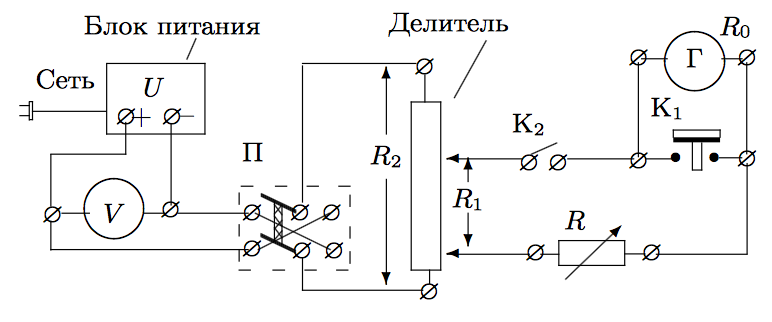
\includegraphics[scale = 0.2]{pic1.png}
\end{center}


\end{abstract}

\pacs{Valid PACS appear here}% PACS, the Physics and Astronomy
                             % Classification Scheme.
%\keywords{Suggested keywords}%Use showkeys class option if keyword
                              %display desired
\maketitle

%\tableofcontent

\section{\label{sec:level1}Резонансная кривая
колебательного
контура}

Для экспериментального исследования резонансной кривой тока в последовательном
колебательном контуре (рис. 1) можно снять зависимость
амплитуды напряжения на резисторе $R$ от частоты генератора (при постоянной амплитуде выходного напряжения генератора). Но импеданс этого
контура включает в себя выходной импеданс генератора. Мы должны быть уверены, что выходной импеданс генератора много меньше импеданса самого контура
и не влияет на процессы, происходящие в контуре.

Для
устранения этого влияния можно использовать схему, представленную
на рис. 2: синусоидальный сигнал с генератора подаётся на параллельный
колебательный
контур через небольшую
разделительную ёмкость
C1. Напряжение с ёмкости
контура C поступает на
вход осциллографа.



Зависимость амплитуды этого напряжения от частоты генератора будет
практически совпадать с резонансной
кривой для последовательного
контура, если импедансы возбуждающей
и
измеряющей цепей намного превосходят импеданс самого контура вблизи
резонанса $Z_{\text{рез}} \approx L/(RC) = Q/(\Omega C)$. Ёмкость
конденсатора $C_1$ выбирается настолько малой, что его импеданс ($Z_{C_1} = 1/(\Omega C_1)$) в рабочем диапазоне
частот много больше импеданса контура, поэтому в цепи генератора течёт ток практически с постоянной амплитудой,
а
колебательный
контур
выполняет роль нагрузочного сопротивления,
которое в свою очередь зависит от частоты.

А так
как сопротивление
$Z_{\text{рез}}$ параллельного
контура
в резонансе максимально, то
и напряжение на ёмкости
$C$ (неизменный
ток, умноженный на максимальное сопротивление) тоже максимально
при резонансе. Входное сопротивление осциллографа достаточно велико:
$R_{\text{эо}} \approx 1$~МOм.

Таким образом, при выполнении
условий:
\begin{equation}\label{1}
    Z_{C_1} = \frac{1}{\Omega C_1} \gg |Z_{\text{рез}}| = \frac{Q}{\Omega C},~~~~R_{\text{эо}} \gg \frac{Q}{\Omega C}
\end{equation}

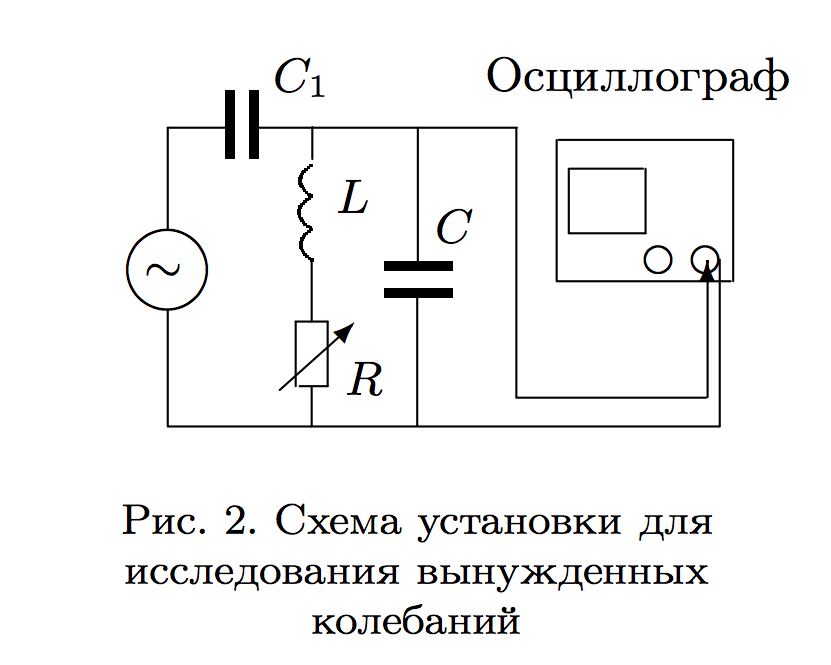
\includegraphics[scale = 0.22]{pic2.png}

и при
условии, что действительная часть импеданса
катушки много меньше её мнимой части, резонансная кривая в нашем
контуре будет выглядеть так
же,
как в последовательном: максимум амплитуды при резонансе. Ширина резонансной кривой определяет важную
характеристику
контура
— \textit{добротность} 
[см. (В.57)].

\section{\label{sec:level1}Процессы
установления
и затухания
колебаний
в
контуре}

Добротность
контура может быть определена
и другими способами,
например, по скорости нарастания амплитуды вынужденных
колебаний при резонансе или по скорости затухания свободных
колебаний.

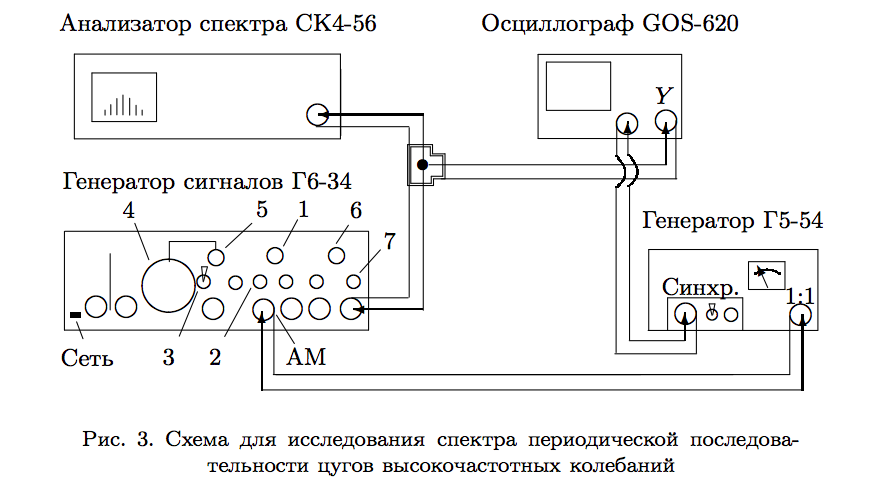
\includegraphics[scale = 0.22]{pic3.png}

Нарастание
и затухание
колебаний
(рис. 3) можно наблюдать на экране осциллографа, если на
контур подаются
цуги — отрезки синусоиды, разделённые интервалами, в течение
которых
сигнал отсутствует. Чем выше добротность, тем медленнее нарастают
и медленнее затухают
колебания в контуре.
Количественные оценки можно сделать,
если определить логарифмический декремент затухания по скорости нарастания или затухания
колебаний [см. (В.30) и (В.73)].
В
условиях резонанса
огибающая затухающих
колебаний
— это перевёрнутая огибающая нарастающего участка. При расчёте логарифмического декремента по затуханию нет необходимости использовать амплитуду
установившихся
колебаний
$U_0$, которая в контуре с высокой добротностью иногда не успевает
установиться за время продолжительности цуга.

\section{\label{sec:level1}Экспериментальная установка}

Схема
установки для исследования
вынужденных
колебаний приведена на рис. 4. Колебательный
контур состоит из ёмкости $C = 0,1$~мкФ, индуктивности $L = 100$~мГн
и переменного
сопротивления
$R$.

Синусоидальное напряжение от звукового генератора про
ходит через
частотомер, позволяющий измерять рабочую частоту с высокой точностью.
В
корпус частотомера вмонтирован генератор цугов
— электронное
реле, разрезающее синусоиду на периодически повторяющиеся цуги
— отрезки синусоиды, содержащие 32 или 40 периодов
колебаний.

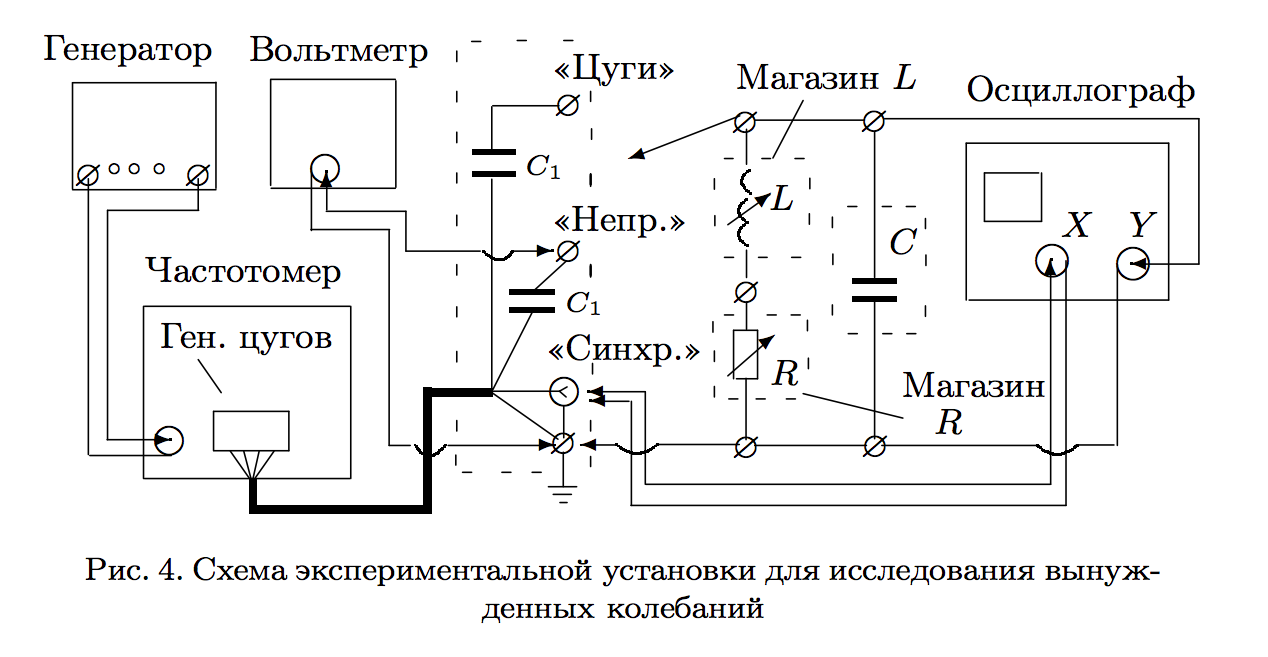
\includegraphics[scale = 0.20]{pic4.png}

После частотомера через небольшую ёмкость $C_1~\approx~600$~пкФ сигнал
поступает на клеммы, смонтированные на отдельной панельке. При подключении контура к клеммам «(земля)» и «Непр» на контур подаётся
непрерывный сигнал — синусоида; если контур подключён к клеммам
«(земля)» и «Цуги» — на контур поступают отрезки синусоиды.

Для наблюдения за процессом колебаний напряжение с ёмкости подаётся на вход осциллографа. Чтобы картина на экране была устойчивой,
частота развёртки осциллографа принудительно синхронизуется с частотой повторения цугов. Для этого на генератор развёртки ЭО подаются
следующие с частотой повторения цугов управляющие импульсы, которые вырабатываются в блоке электронного реле (клемма «Синхр», смон-
тированная на панельке). Для измерений напряжения на ёмкости используется электронный вольтметр.

\section{\label{sec:level1}Задание}

В работе предлагается при двух значениях сопротивления магазина
($R = 0$ и $100$ Ом) исследовать резонансные кривые и определить по ним
добротность контура; затем рассчитать добротность, определив логарифмический декремент затухания при нарастании и при затухании колебаний.

\begin{center}
\textbf{Подробно правила выполнения работы изложены
в ДОПОЛНИТЕЛЬНОМ ОПИСАНИИ,
расположенном на установке.}
\end{center}
1. Соберите схему по рис. 4 и подготовьте приборы к работе.\\
2. Установите на магазине индуктивностей $L = 100$ мГн и рассчитайте резонансную частоту контура по формуле $\nu_0 = 1/(2\pi \sqrt{LC})$.\\
3. Исследуйте резонансные кривые контура [$U_C~=~f(\nu)$] для сопротивлений
$R = 0$ и $R = 100$~Ом.\\
4. Определите добротность контура по нарастанию и затуханию колебаний
для $R = 0$ и $R = 100$~Ом, для этого переключите контур на вход «Цуги»
и установите резонансную частоту.\\
5. Сместите частоту генератора с резонансного значения и получите на
экране картину биений. Зарисуйте и объясните её.\\
6. Измерьте активное сопротивление $R_L$ магазина индуктивностей c помощью моста Е7–8.
\begin{center}
Обработка результатов.
\end{center}
1. Постройте на одном графике резонансные кривые в координатах $U / U_0 = f(\nu/\nu_0)$, где $U_0$ — напряжение при резонансной частоте $\nu_0$.

Определите добротность по формуле (В.57). Сравните теоретическое
и экспериментальное значения резонансной частоты.\\
2. Рассчитайте добротность контура по скорости нарастания и затухания
колебаний (см. (В.30), (В.31) и (В.73)).\\
3. Рассчитайте теоретическое значение добротности через параметры контура $L$, $C$ и $R$ (см. (В.28)).\\
4. Сведите результаты определения $Q$ в таблицу.
5. Оцените погрешности измерений и сравните результаты расчётов $Q$.
\newpage
\section{\label{sec:level1}Обработка измерений}

1. Посмотрим на графики резонансных кривых в координатах $U/U_0~=~f(\nu/\nu_0)$. Измерения проводились так, что значению $\nu_0$ соответствует измерение $U_0~=~10~\text{дел}$. 

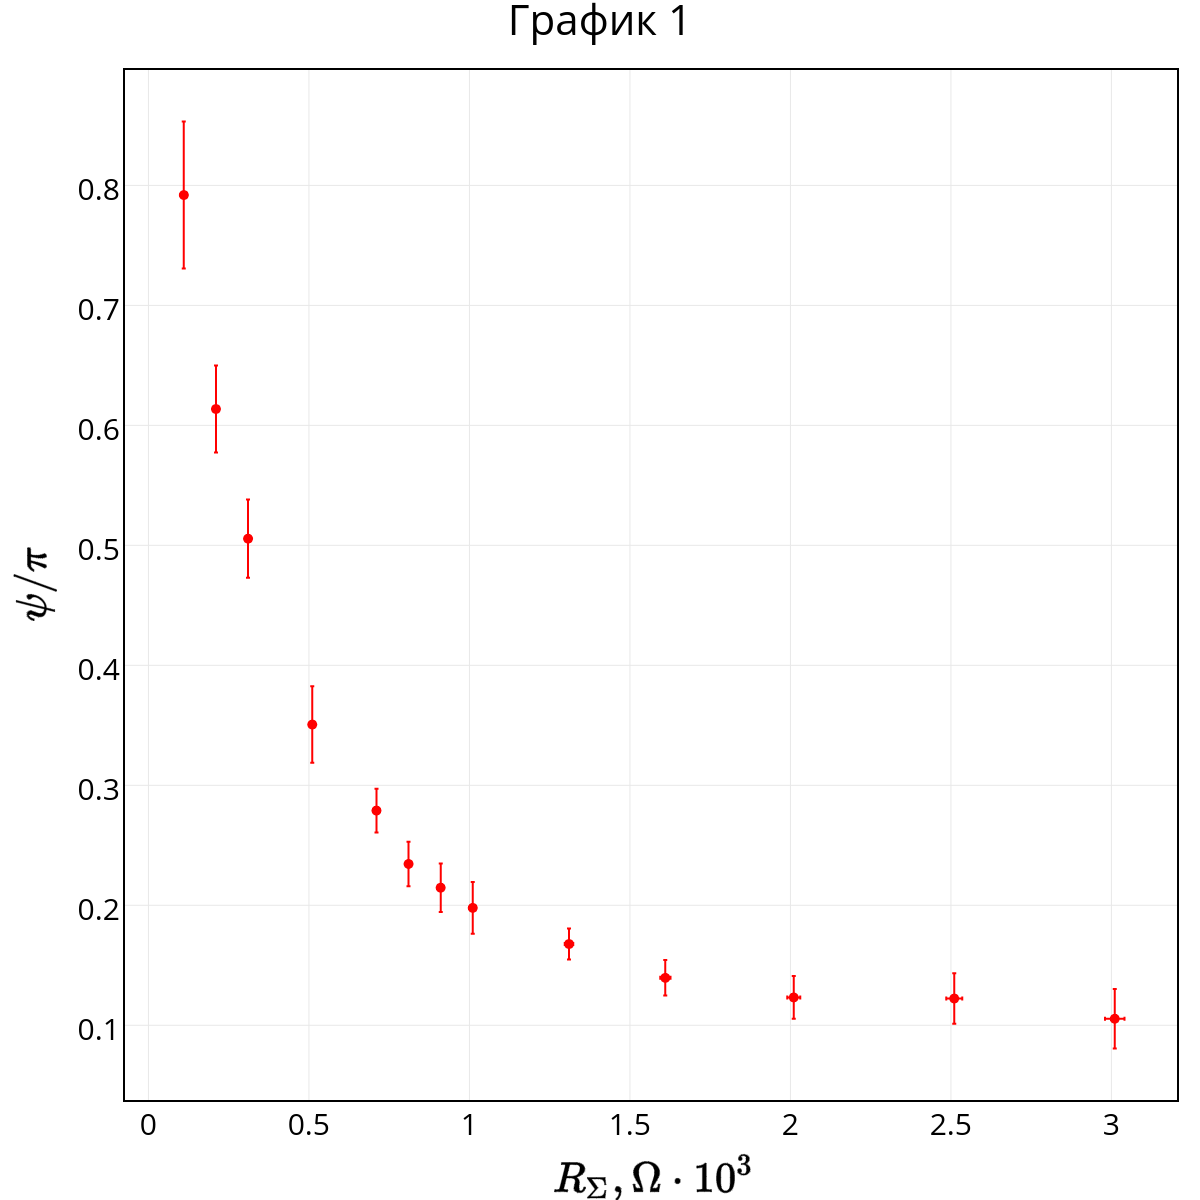
\includegraphics[scale = 0.19]{my_plot1.png}

Теперь определим добротность для двух значений $R$. Построим графики для этих значений и обозначим линию уровня соответствующую значению $U~=~U_0/\sqrt{2}$. 

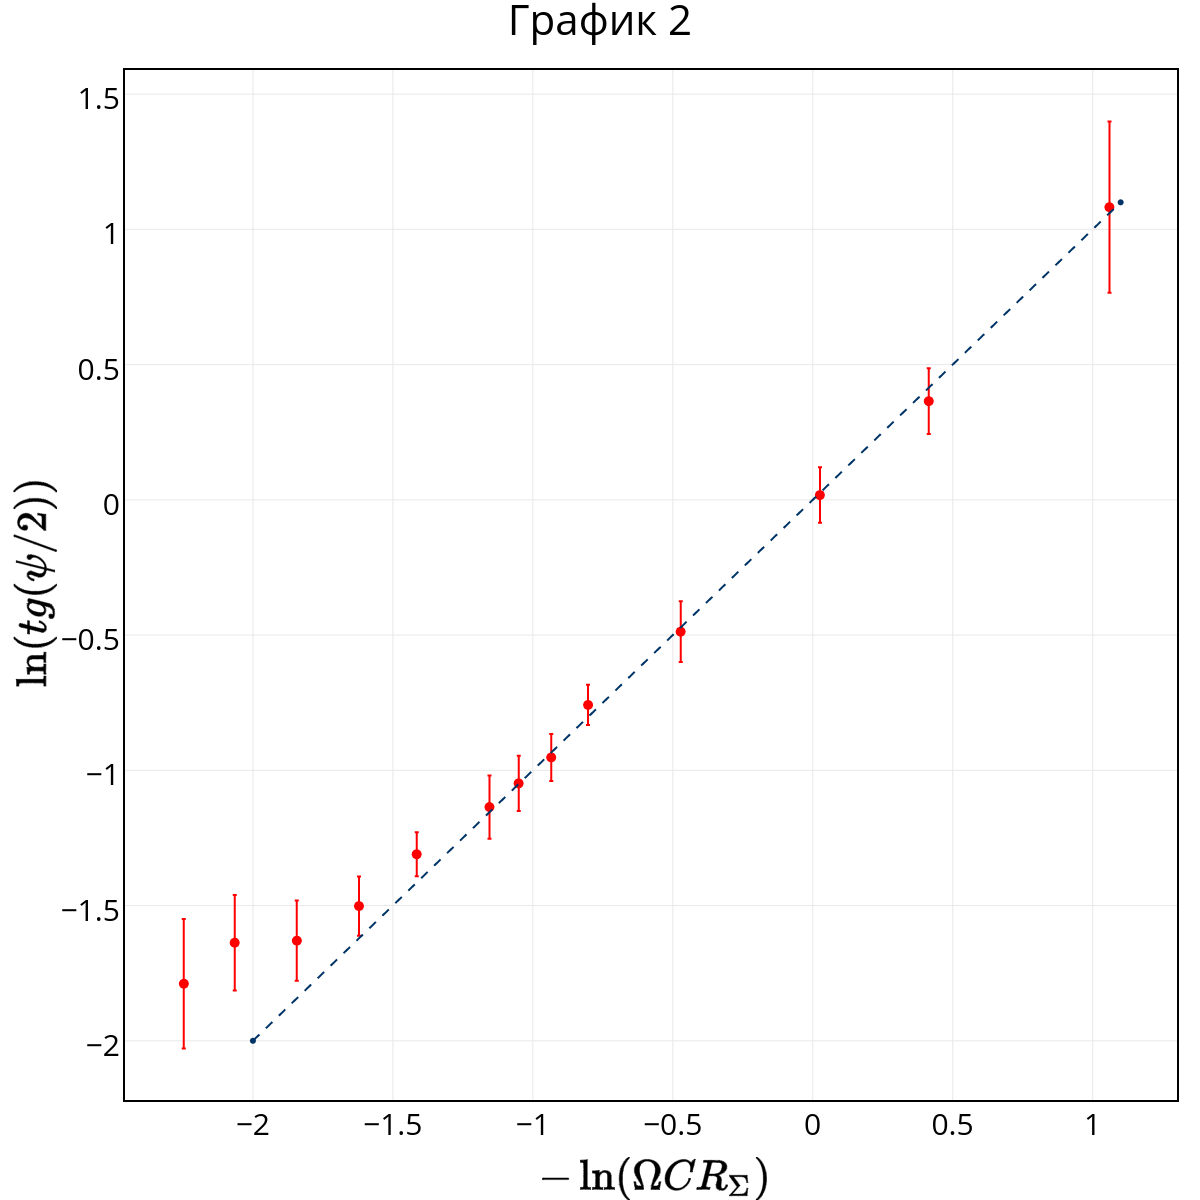
\includegraphics[scale = 0.19]{my_plot2.png}

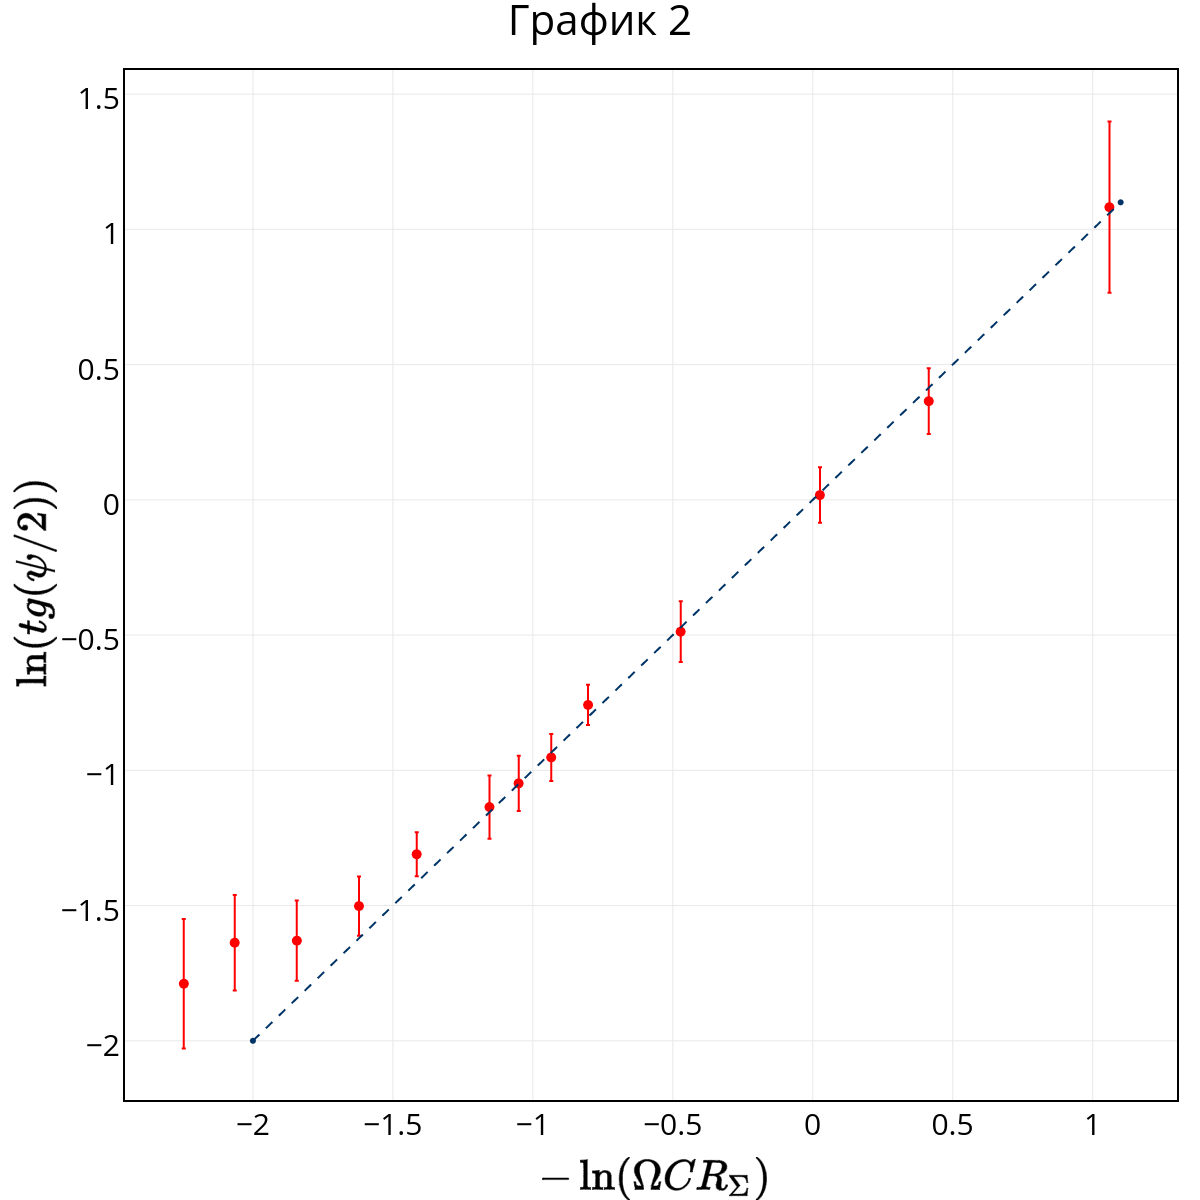
\includegraphics[scale = 0.19]{my_plot2.png}

Далее, вероятно, более правильным методом является построение нелинейной модели и минимизация функционала ошибки, с помощью этого метода можно получить оценку на значение добротности исключительно из параметров модели. Однако в работе предлагается другой подход, а именно: линейно интерполируем резонансную кривую на всём промежутке измерений, найдём пересечение с заранее обозначенной линией уровня и найдём значение ширины резонанса на уровне $U_0/\sqrt{2}$. Оценим ошибку измеренной величины таким способом. Результат занесём в итоговую таблицу.

Далее проведём анализ скорости нарастания и затухания колебаний. По предложенным в описании формулам вычислим по три значения для 4 серий измерений, усредним и оценим ошибку. 
$$ \Theta^{\text{up}} = (0.11 \pm 0.01) $$
$$ \Theta^{\text{down}} = (0.09 \pm 0.01) $$
$$ \Theta^{\text{up}}_{\text{R}} = (0.32 \pm 0.02) $$
$$ \Theta^{\text{down}}_{\text{R}} = (0.34 \pm 0.01) $$

\newpage
Параллельно рассчитаем теоретическое значение добротности через параметры контура $L,~C~\text{и}~R$.

Итого:
\\
\\
\\
\\
\\
\\
\\
\\
// Данная лаба была доделана в оффлайн режиме. Сорян за мою ленность и тупость.
\\
\\
\\
\\
\\

\newpage
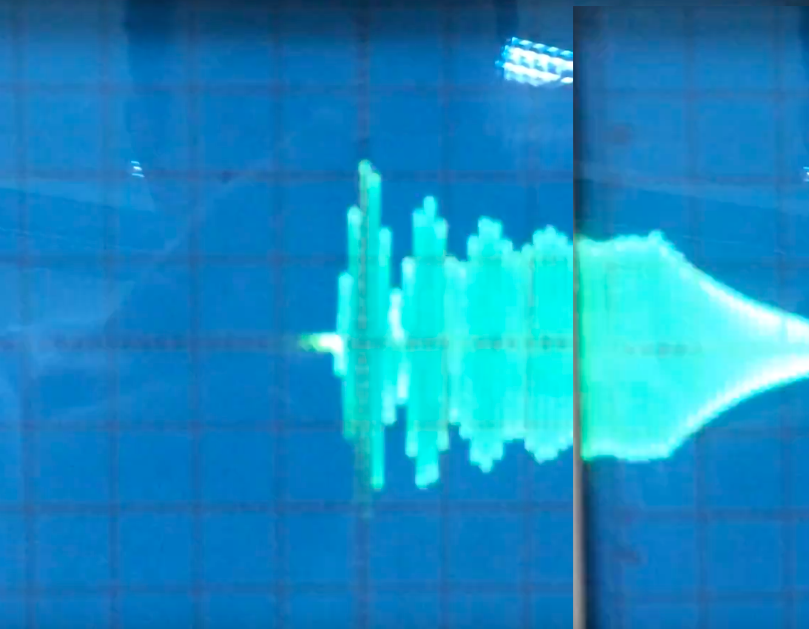
\includegraphics[scale = 0.30]{my_photo.png}



\end{document}

